\documentclass{article}

\usepackage{graphicx} % for images
\usepackage{amsmath} % for math
\usepackage{amssymb} % for \mathbb
\usepackage{siunitx} % for \SI, \num
\usepackage{hyperref} % for \url{}

% This stuff is for figures
\usepackage{float}
\DeclareGraphicsExtensions{.pdf, .png, .jpg}

% coloring of links for PDF format
\hypersetup{
    colorlinks=true,
    urlcolor=blue,
    linkcolor=black
}

% \c command redefinition (for monospaced font)
\renewcommand{\c}[1]{\texttt{#1}}
% \today command re-definition
%https://tex.stackexchange.com/questions/112932/today-month-as-text
\renewcommand{\today}{\ifnum\number\day<10 0\fi \number\day \space%
\ifcase \month \or January\or February\or March\or April\or May%
\or June\or July\or August\or September\or October\or November\or December\fi\space%
\number \year} 

\begin{document}
\begin{titlepage}
	\centering
	
\includegraphics[width=0.25\textwidth]{Images/247px-CSU-Longbeach_seal}\par\vspace{1cm}
	{\scshape\Large California State University, Long Beach \par}
	\vspace{1cm}
	{\scshape\Large CECS 447\par}
	\vspace{1.5cm}
	{\huge\bfseries Project 1\par}
	\vspace{2cm}
    {\Large\itshape Rodrigo Becerril Ferreyra\par}
    {\itshape\Large Student ID 017584071 \par}
	\vfill
    A project that uses the ARM Cortex-M4 microcontroller to
    play music.

	\vfill

% Bottom of the page
	{\large \today\par}
\end{titlepage}

\section{Introduction} The purpose of this project is to play
music using a microcontroller. The project is split into two
parts: first, using a digital output (square wave) to drive
a speaker, and then using an analog output (sine wave) coupled
to a passive digital-to-analog converter (DAC).

\section{Operation}
Since this project was split into two parts, I will describe the
operation of both parts separately.

\subsection{Part 1}
The first part brings the task of driving a speaker by sending
square waves to the speaker; that is, it uses one GPIO pin to
drive the speaker, and it is turned on and off. The frequency of
the note played is equal to double the frequency that the output
flips its value; if the output switches at a frequency of
\SI{440}{\hertz}, then the note played will be of a frequency of
\SI{880}{\hertz}.

We are using the SysTick timer to control the frequency of each
note played. Assuming a default system clock rate of 16 million
cycles per second (\SI{16}{\mega\hertz}), the formula to find
the reload value for the SysTick timer comes out to be
\begin{equation}\label{eq:reload part 1}
	v_1 = \frac{\SI{16}{\mega\hertz}/f_\text{note}}{2}-1
\end{equation} where \(v_1\) is the reload value and
\(f_\text{note}\) is the frequency of the desired note.

The main function of Part 1 is to play three songs: the Happy
Birthday song, Marry Had a Little Lamb, and Twinkle Twinkle
Little Star. The song that's currently playing loops indefinitely
until one of the buttons are pressed: the left button starts or
stops the song, while the right button changes the song.

Here is a video detailing the operation of Project 1 Part 1:
\url{https://youtu.be/ltoyG6DEJn0}

\subsection{Part 2}
For Part 2, instead of driving the speaker with a square wave,
the task at hand is to output a six-bit sine wave. The sine
wave is to be outputted in 64 discrete intervals per
\(360^\circ\) of sine wave. This necessitates a DAC, to convert
a digital number from 0 to 63 into an analog voltage to drive
the speaker.

Instead of using an IC DAC circuit that uses serial
communication, I used an R-2R passive resistor ladder DAC circuit
instead. This simplicity comes with the tradeoff of having to
amplify the output before it is able to drive the speaker.

Since the output changes 64 times per sine cycle, the new
reload value \(v_2\) changes into
\begin{equation}\label{eq:reload part 2}
	v_2 = \frac{\SI{16}{\mega\hertz}/f_\text{note}}{64}-1
\end{equation}

In addition to this, Part 2 has two modes: a music box mode
similar to Part 1, and a piano mode. In the music box mode,
the right button changes the song, and the left button switches
to piano mode.

In piano mode, the system takes input from four buttons; these
play the notes C, D, E, and F in the octave that is currently
selected. The right button changes octave (there are three total),
and the left button switches back to music box mode. Note that
the songs played in music box mode will be played in the
selected octave (the program remembers the octave it was in).

Here is a video detailing the operation of Project 1
Part 2 when in music box mode:
\url{https://youtu.be/4n18laB_mus}

Here is a video detailing the operation of Project 1
Part 2 when in piano mode: \url{https://youtu.be/qKPznZU5S7s}

\section{Theory}
Since we are already using the SysTick timer to control the
frequency of the note being played, we have to rely on a
software loop to control the duration of the note (using a
general-purpose timer would be overengineering, since the
complexity it would add would supersede the benefits).

\section{Hardware Design}
The speaker I am using is rated at \SI{4}{\ohm} up to \SI{3}{\watt}.
The low impedance posed a serious problem in the second part,
since I am rather unexperienced with amplifiers and amplification.
It took me a lot of work to create an emitter follower with the
small-signal transistors and low-power resistors I have at hand.
Figure \ref{emitter follower} is the emitter follower I have
built. \(V_\text{in}\) represents the output of the DAC, which
is a sine wave with \SI{3.3}{\volt} peak-to-peak and a DC offset
of \SI{1.65}{\volt} at \SI{440}{\hertz}.

\begin{figure}[H]
	\centering
	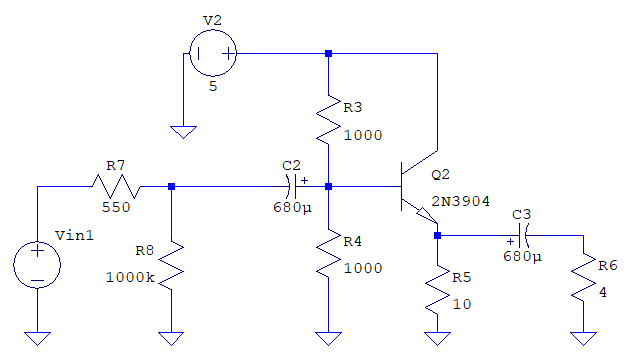
\includegraphics[width=\textwidth]{Images/EmitterFollower}
	\caption{Low-power emitter follower.}
	\label{emitter follower}
\end{figure}

The resulting output has a voltage of about \SI{282.84}{\milli\volt}
and \SI{70.71}{\milli\ampere}, which is a power output of
approximately \SI{20}{\milli\watt}. This is audible to the
ear in a standard environment, but this is much quieter than
other students' pre-built amplifiers, and it is hard to hear
through Zoom (so much that I had to put the microphone directly
on the speaker so it would pick up the speaker's vibrations).
I could make this amplifier
much louder if I had a power BJT and some high-power resistors
at hand.

Figures \ref{part 1 schematic and pic} and
\ref{part 2 schematic and pic} detail the hardware schematics
and embedded system pictures of Parts 1 and 2, respectively.

\begin{figure}[H]
	\centering
	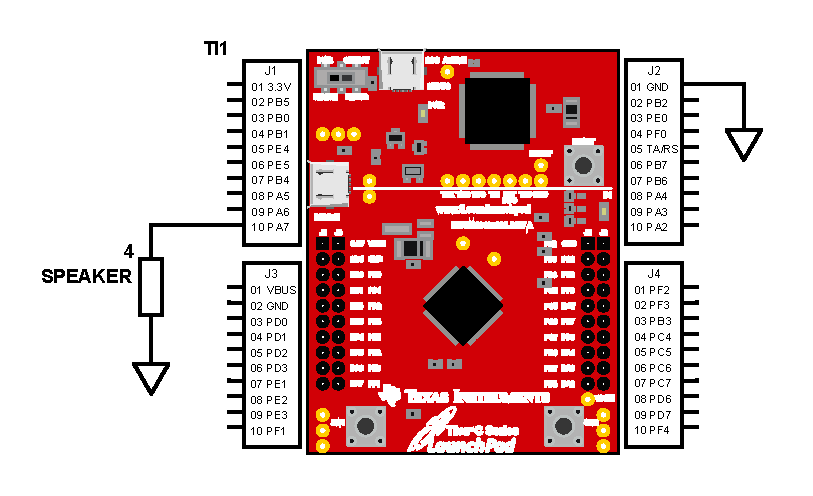
\includegraphics[width=\textwidth]{Images/Part1Schematic}

	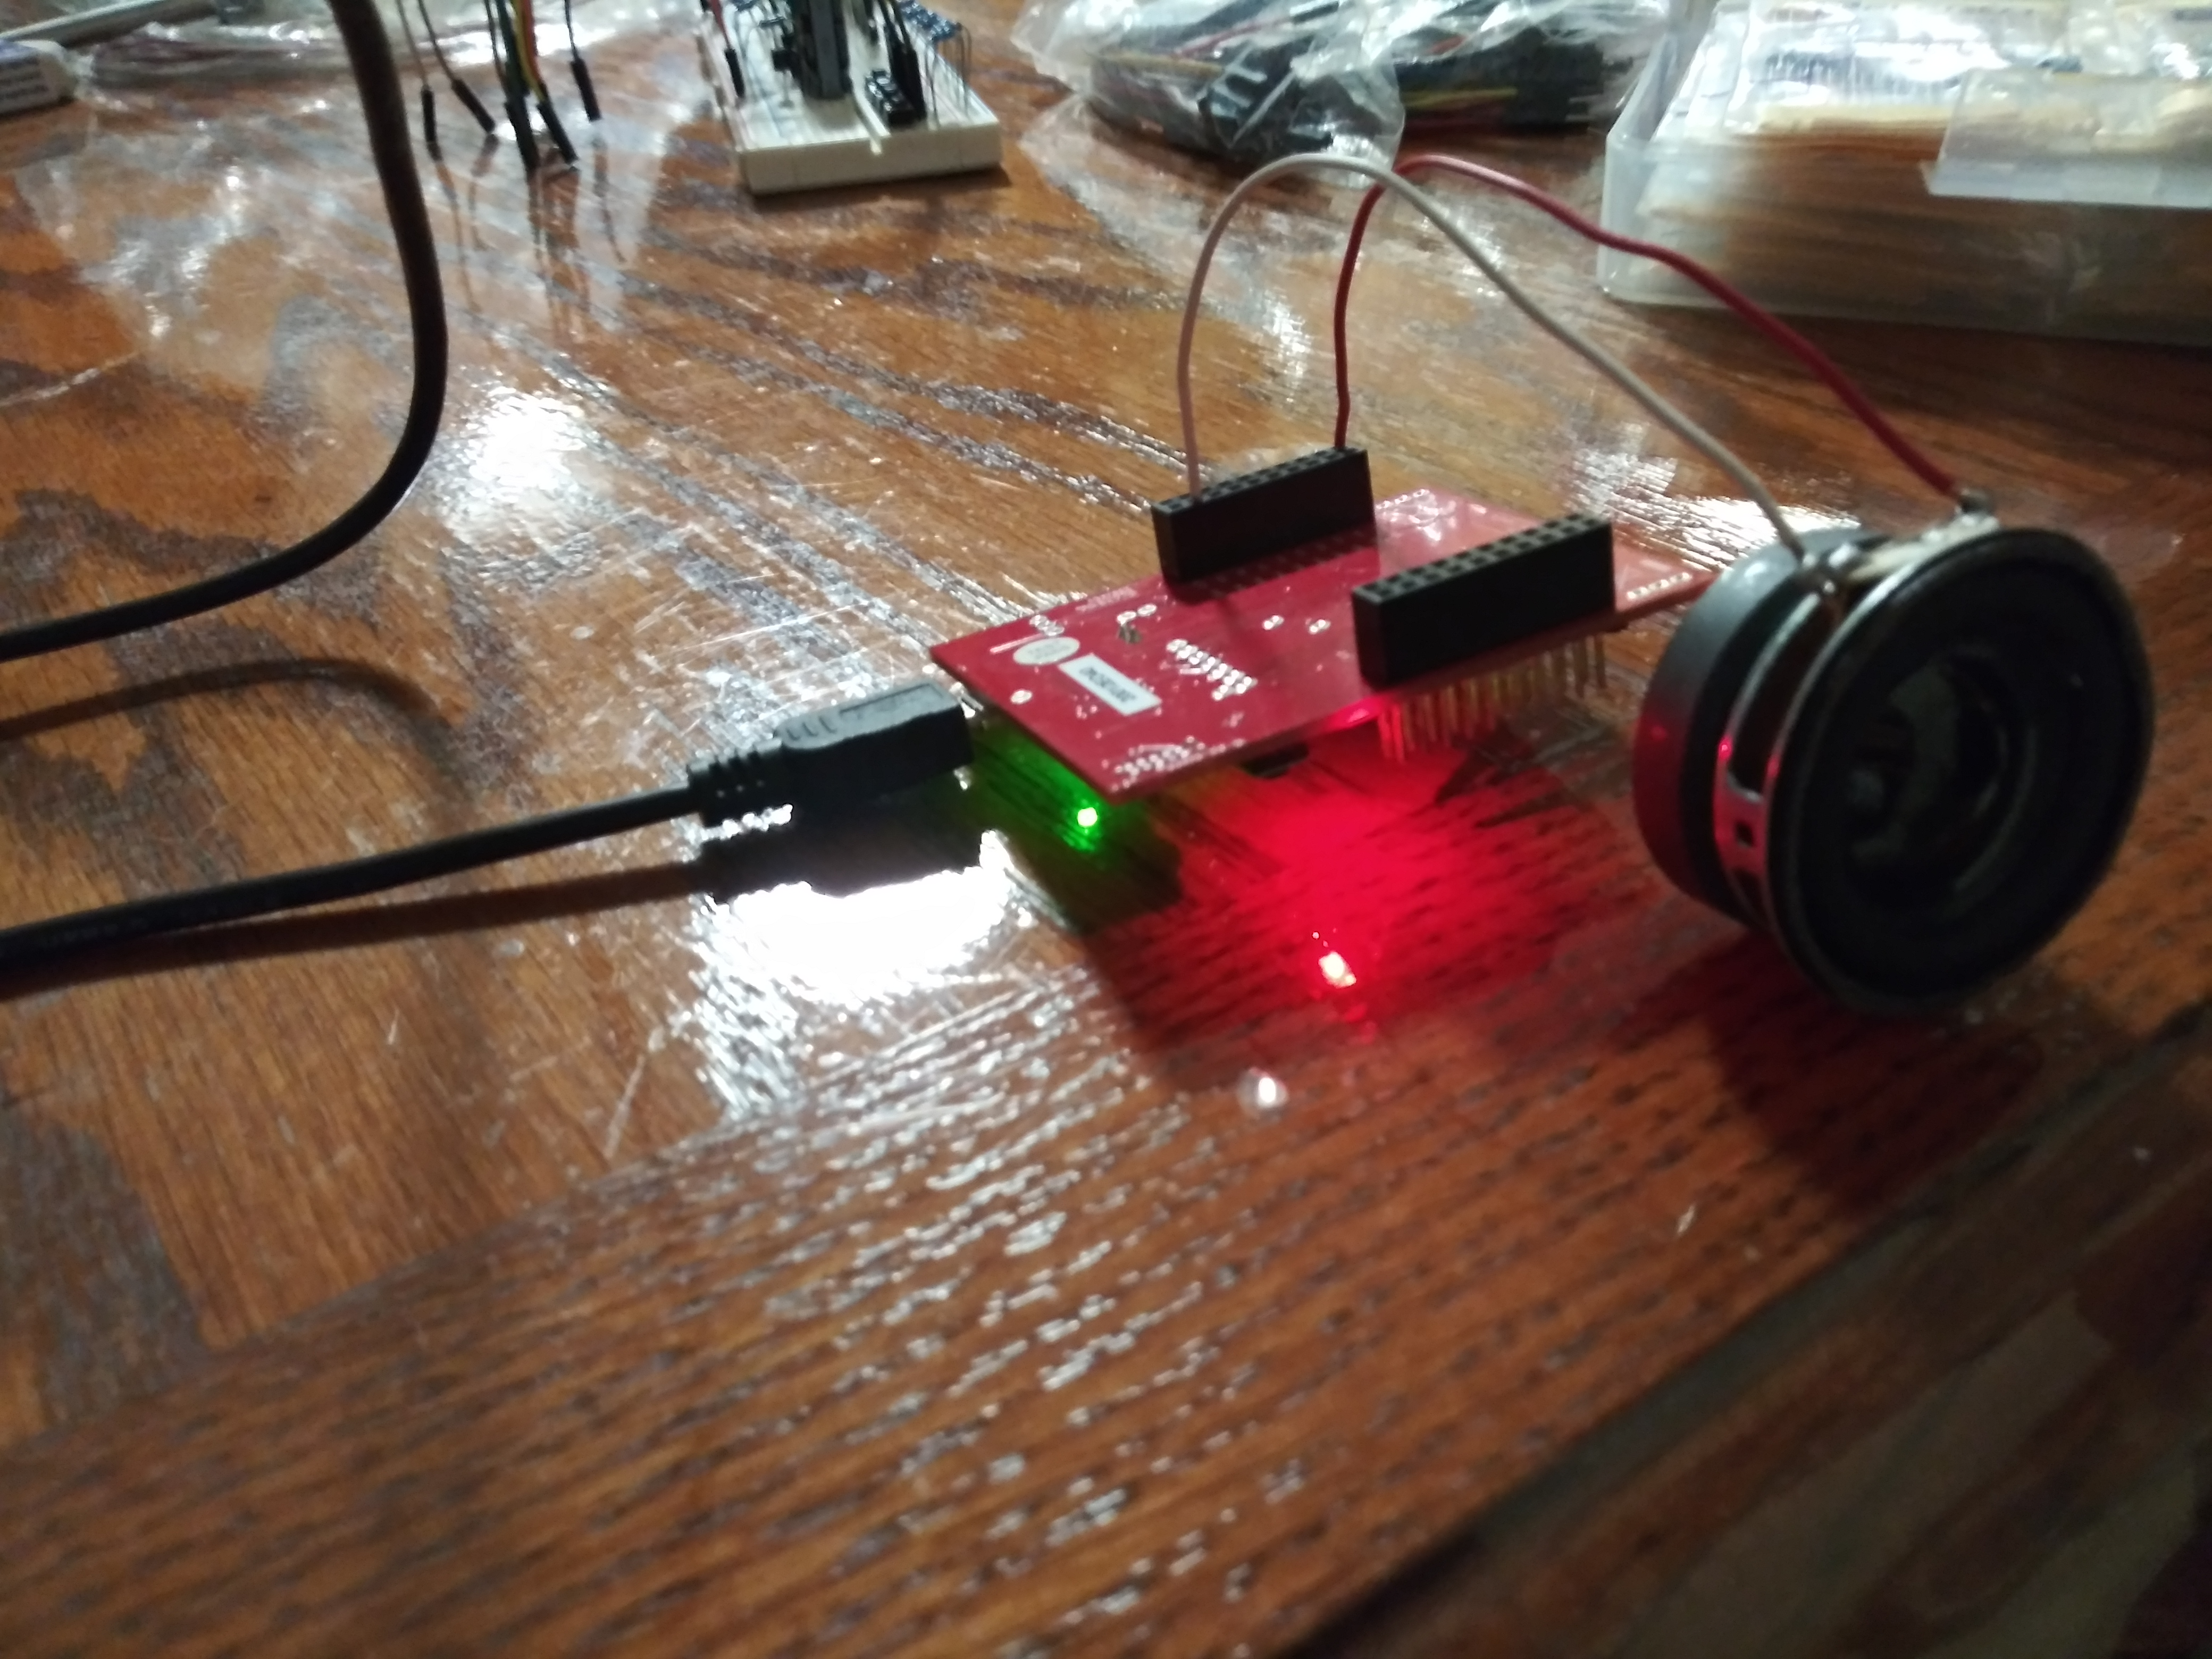
\includegraphics[width=\textwidth]{Images/Part1System}
	\caption{Schematic diagram and picture of Part 1 implementation.}
	\label{part 1 schematic and pic}
\end{figure}

\begin{figure}[H]
	\centering
	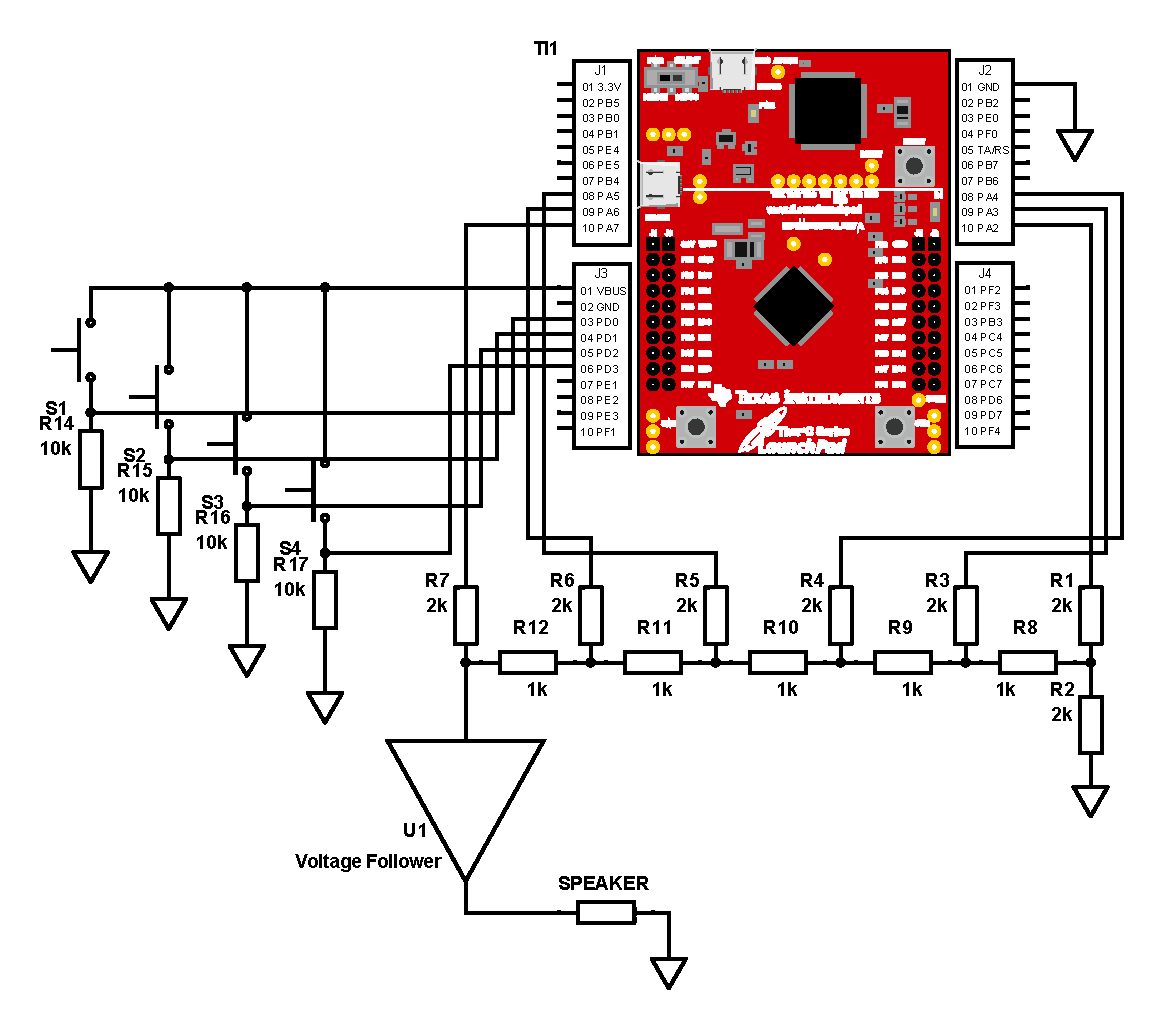
\includegraphics[width=\textwidth]{Images/Part2Schematic}

	\includegraphics[width=\textwidth]{Images/Part2System}
	\caption{Schematic diagram and picture of Part 2 implementation.}
	\label{part 2 schematic and pic}
\end{figure}

\section{Software Design}
I used structs to define a \c{Note}, which have a reload value
and an amount of time to hold. Each song is an array of
\c{Note}s; to play the song, a function loops through this
array, sets the SysTick timer's reload register to whatever the
\c{Note} requires, and turns the timer on. The timer stays on
until the software loop finishes (i.e. until the correct time
as defined by \c{Note} has elapsed). There is a special "note"
which signifies the end of song, in which case the same song is
repeated.

The on-board buttons trigger interrupts to perform
different tasks, depending on the Part: they can force the
song to stop playing, change song, or change octave. The on-board
LEDs are signals that signify different things: in Part 1,
the red LED turns on when the output is high and turns off when
the output is low; in piano mode, the LED is blue when the program
is in piano mode, and red when the program is in music box mode.

\section{Conclusion}
This first project is more like two, and it brings many
old and new concepts together. I had much trouble with the
voltage follower. I also had trouble with my notes being out
of pitch during the live demo, though they sound better in
the video. Overall, this was a challenging but fair project.

\end{document}
